\documentclass[bibliography=totoc]{scrartcl}
\usepackage[ngerman, english]{babel}
\usepackage{rwukoma}
\usepackage[pdfusetitle]{hyperref}
\usepackage{lipsum,caption}
\usepackage{acronym}
\usepackage{algorithm, algpseudocode}
\usepackage{graphicx}
\usepackage{subcaption}
\usepackage{listings}
\usepackage{float}
\usepackage{todonotes}
\usepackage{amsmath}
\usepackage{comment}

\setlength{\belowcaptionskip}{5pt}

\title{Comparison path planning algorithms}
\author{Manuel Gnannt - 34946, IN \\ Florian Betz - 35653, IN}
\date{13.03.2023}%\today}
\begin{document}
\maketitle
\tableofcontents

\clearpage
\section{Abstract}
In path planning, discovering good trajectories often requires a high-dimensional model and the evaluation of many samples. Recently, Wang et al. proposed an algorithm called \textbf{La}tent Space \textbf{P}artitions for \textbf{P}ath \textbf{P}lanning (LAP3) claiming it outperforms existing path planning methods in 2D navigation tasks with respect to sample efficiency. In this paper, we compare the newly published LAP3 to other path-planning algorithms in several 2D environments.
\todo[inline]{extend descriptions with all information}
\todo[inline]{problems, why, solutions, results}

\section{Introduction}
In path planning, the goal is to find the most rewarding trajectory (represented as a sequence of actions at a given state) in a given search space. 

Common problems of path planning algorithms include being trapped at local optima or the exploration-exploitation tradeoff.
Different applications require different search algorithms.
An algorithm that works well in one scenario may be inefficient in another. 
Additionally, the branching factor of a problem can greatly affect the computation time, making it necessary to use specialized search algorithms to handle large branching factors. 
Furthermore, completeness is an important consideration for search algorithms, as it ensures that the algorithm can always reach the goal. 
Finally, when searching for an optimal solution, it is necessary to find the solution with the lowest cost, which requires specialized algorithms.

To tackle these problems, Wang et al. proposed LAP3 \cite{NEURIPS2021_03a3655f}, an algorithm which partitions the search space into high- and low-reward regions. These regions are represented in a monte-carlo tree and the path from the current node to the goal is computed.

The algorithm differs in the way it takes the samples and partitions the search space. While other path-planning algorithms such as La-MCTS \cite{DBLP:journals/corr/abs-2007-00708} partition the search space based on a few samples and then take additional samples afterwards, LAP3 takes samples first and then recursively partitions the search space based on a minimal number of samples per region.

This paper explores the topic of path planning, with a focus on three specific algorithms A*, LaMCTS, and LaP3. 
Path planning is an important aspect of robotics and artificial intelligence, as it enables robots and other autonomous systems to navigate through an environment and reach a desired destination. 
The A* algorithm is a well-known and widely used method for pathfinding and graph traversal, which incorporates heuristic functions and predicted costs to find the most efficient path. 
LaMCTS and LaP3, on the other hand, are more recent algorithms that have been developed to address specific challenges in path planning, such as handling large or complex environments.

\section{Evaluation Criteria} \label{corner_detection}
\todo[inline]{short description}

\begin{comment}
    
\subsection{Space Complexity}
Space complexity is a metric that expresses the amount of temporary storage space utilized by an algorithm during its execution. 
It is represented as $O(f(n))$, where $f(n)$ is the function that describes the storage space required by the algorithm. \cite[p. 303]{TheoryComputation}
The amount of temporary storage space used during runtime can differ between different algorithms. 
Some algorithms only require a minimal amount of temporary space and remain constant regardless of the size of the problem and are called "in-situ" which means space-efficient. 
While other algorithms use multiple temporary work units that are related to the size of the problem, represented as n, and increases as n increases. 
When n is large, more storage units will be utilized, resulting in a higher space complexity.
\end{comment}

\subsection{Search Efficiency}

Global path planning algorithms create paths based on pre-existing information, while local path planning algorithms generate paths by gathering information about the environment via a sensor. 
Regardless of the algorithm, it must possess the capability to react quickly to environmental information, have low computational requirements and short search time, and have high search efficiency. Different algorithms exhibit varying levels of search efficiency.

\subsubsection{sample-reward ratio}
\todo[inline]{descripte criteria, Manuel}
\subsubsection{function evals reward ratio}
\todo[inline]{descripte criteria}

\newpage
\section{Path Planning Algorithms}
\label{path_planning_algorithm}
In this paper, we decided to use three different search algorithm A*, \ac{MCTS} and \ac{LaP3}.

\subsection{A*}
\todo[inline]{image? Florian}
The A* algorithm, first introduced by Peter Hart and other researchers at the Stanford Research Institute in 1968, is a widely used method for pathfinding and graph traversal. \cite{4082128} It builds on Dijkstra's algorithm by incorporating heuristic functions and predicted costs, making it the most efficient direct search method for finding the shortest paths in a static road network and a popular heuristic for various other problems.\cite{ProbabilisticApproachCollaborativeMultiRobotLocalization}

The key component of the algorithm is the design of the valuation function, $f(n) = g(n) + h(n)$, where $g(n)$ is the actual cost from the initial node to node n, $h(n)$ is the estimated cost from node n to the target node, and $f(n)$ is the estimated cost from the initial node via node n to the target node.

The steps of the A* algorithm are:

\textbf{Step 1:} Add the starting node to the priority queue.

\textbf{Step 2:} Select the node with the smallest F-value from the current priority queue and make it the current node.

\textbf{Step 3:} Mark it as visited and process its adjacent nodes.

\textbf{Step 4:} If the neighboring node has not been visited, add it to the queue, set the current node as its parent, and record its F, H, and G values. If the neighboring node has already been visited, check if the current node has a shorter path by comparing G values. If the current node has a smaller G value, update the parent node and G, H values of that node.

\textbf{Step 5:} Repeat steps 2 to 4 until the target node is marked or the priority queue is empty.

\textbf{Step 6:} When the path is found, trace back from the endpoint to the start node using the parent node.

The A* algorithm can reach a time complexity of $O(n)$.

\subsection{Monte-Carlo Tree-Search}
\todo[inline]{unbedingt notwendig?}
The leaves in the monte-carlo tree represent different states in a search space. The links to different children of a leaf represent different actions to get to a different state.

\begin{figure}[H]
	\centering
	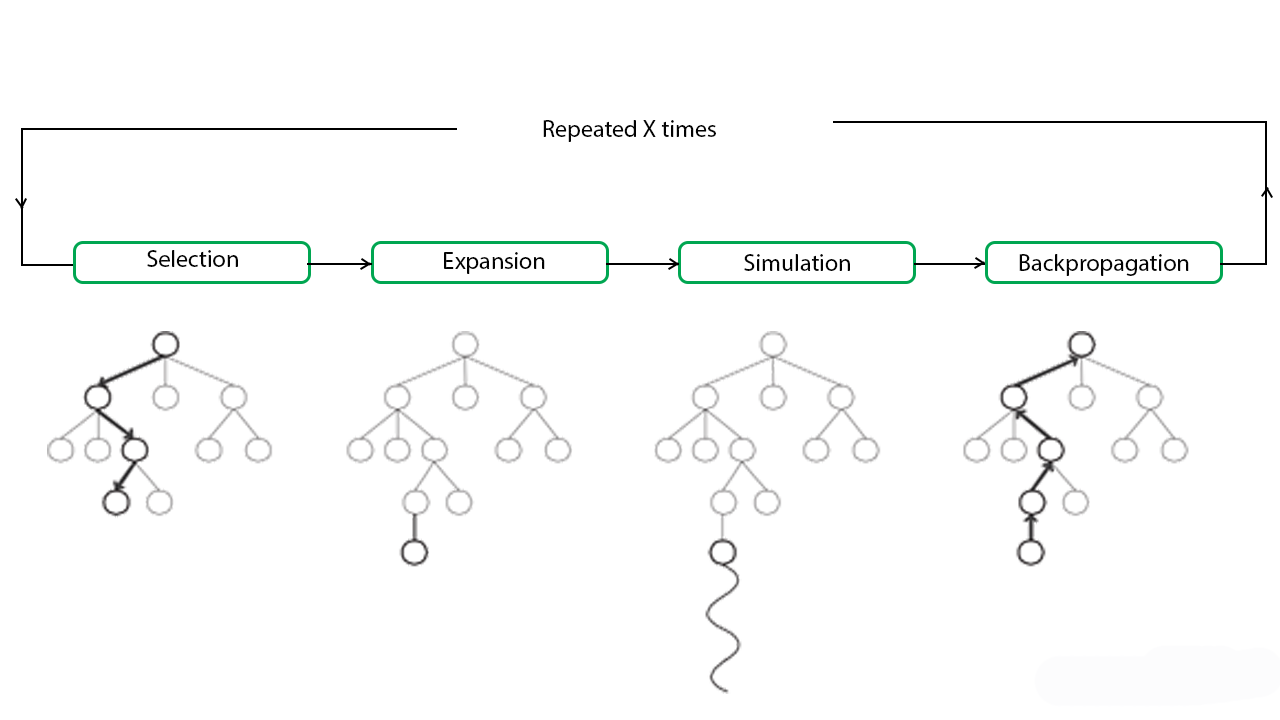
\includegraphics[width = {\textwidth}]{img/mcts_steps.png}
	\caption{Steps of \ac{MCTS}}
	\label{fig:MCTS}
\end{figure}

The tree now learns by performing the following steps:

\textbf{Step1: Selection} When in a given state, an appropriate action is selected based on a policy.

\textbf{Step 2: Expansion} When the selected leaf does not have any children, different actions are performed which lead to additional nodes.

\textbf{Step 3: Simulation} The reward of the newly created leaves is calculated and the best nodes are added to the tree.

\textbf{Step 4: Backpropagation} All nodes above the selected one are updated based on the reward they lead to.

\subsection{LaMCTS}
\todo[inline]{Schreieben Manuel!}
In a Latent space Monte-Carlo Tree-search, the search space is represented using a monte carlo tree. This is done by taking samples and splitting the search space in a high-reward partition and a low-reward partition using k-keans(k=2) and an SVM learning the boundary. These partitions are represented by two child nodes in the monte-carlo tree. In a next step, samples are taken from around each cluster center and based on these samples, the now child-node is partitioned again in a high- and low-reward region. This results in a monte carlo tree with the left-most leaf being the highest-reward region, the leaf left to the highest one being the second-highest and so on.
\begin{figure}[h!]
    \centering
    \begin{subfigure}[b]{0.3\linewidth}
    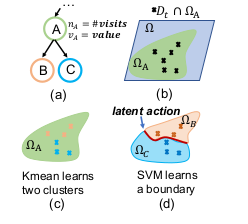
\includegraphics[width=\textwidth]{img/lamcts_1.png}
    \caption{La-MCTS sampling and splitting \cite{DBLP:journals/corr/abs-2007-00708}}
    \label{fig:mesh1}
    \end{subfigure}
    \hspace{0.02\textwidth}
    \begin{subfigure}[b]{0.3\linewidth}
    \centering
    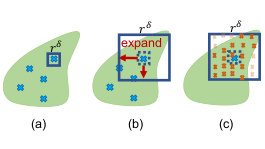
\includegraphics[width=\textwidth]{img/lamcts_2.png}
    \caption{La-MCTS sampling around cluster center \cite{DBLP:journals/corr/abs-2007-00708}}
    \label{fig:mesh1}
    \end{subfigure}
\end{figure}

\todo[inline]{verweis auf paper quelle, indem der MCTS beschrieben wird}

\begin{comment}
\subsubsection{Selection}
With the help of an evaluation function (heuristic), the selection of a node s follows. 
However, it should be noted that non-preferred nodes should also be considered.
In some cases, the non-preferred nodes may have a higher value.With the help of an evaluation function (heuristic), the selection of a node s follows. 
However, it should be noted that non-preferred nodes should also be considered.
In some cases, the non-preferred nodes may have a higher value.

\subsubsection{Expansion} 
In this step, the children of the selected node s are considered. 
If there are one or more children that have not yet been expanded, these children are added to the search tree.
These children are added to the search tree. 
However, if all children of the nodes have been expanded, then another or also a child node s is selected and
the expansion step is then executed on the nodes.

\subsubsection{Simulation} 
The search policy follows from this step. Here, playouts are executed on the newly added child nodes.
child nodes that have been added. There are also two options for the playout.
One chooses purely random moves without knowing the rules of the game.
One uses a heuristic so that there is less randomness present
Looking at the last moves, which lets you know beforehand if you missed/achieved the goal).
In a nutshell, it means that from the newly added child node to a hand
random moves are chosen.

\subsubsection{Backpropagation}
Finally, the last step Backpropagation occurs. After a leaf is reached by the simulation, all nodes in the search tree are updated.
In addition, for each node j traversed, the simulation number nj is incremented by one is increased.
\end{comment}

\subsection{LaP3}
The LaP3 algorithm works similar to La-MCTS. Contrary to La-MCTS, Samples are collected at the beginning and the search space is then split recursively into good and bad regions until a threshold of samples is undercut.

\todo[inline]{write LaP3 algorithm!!! Manuel}
The \ac{LaP3} algorithm is an extension of the LaMCTS. \cite{NEURIPS2021_03a3655f}
It is a new path planning method which improves the function value estimation within each sub-region.
This algorithm use a latent representation of the search space.
\ac{LaP3} and \ac{LaMCTS} use the maximum, instead of the mean, as the node score to improve sample efficiency.

\newpage
\section{Methodology}
A common problem of path planning is being trapped in local minima[...] thus suitable environments were selected for the algorighms

We ran all 3 algorithms on two different environments (mazes3, 4 rooms)
\todo[inline]{Was haben wir haben? Manuel}
\todo[inline]{Warum haben wir es gemacht? Manuel}
\todo[inline]{environment description Manuel, Maze s3 and four rooms images Florian}
\newpage
\section{Evaluation}

\todo[inline]{Write short introduction into the chapter, Florian}
\todo[inline]{Astar mit anderem Verzweigungsfaktor}
\todo[inline]{mehr Daten damit Astar mit MCTS und LAP3 besser verglichen werden}
\todo[inline]{if lenyvec good größer 5 wie viele samples pro region immer beide ändern}
%\todo[inline]{MCTS in LaMCTS abändern}


%1. LaP3 Algorithmus wurde entwickelt, der die Pfade schneller berechnet
%2. LAP3 performt besser als der MCTS und A*
%3. Anhand gleicher Anzahl an samples ist der reward beim LAP3 immer besser
%4. verschiedene Metriken wurden verwenden space complexity, world environment
%5. Was sind unsere Ergebnisse, Performt LAP3 tatsächlich immer besser?
%6. Was kann in Zukunft noch nageschaut werden?

When each algorithm is run, the maximum reward to be achieved is compared to the number of samples taken. As this result can vary, each algorithm is run 100 times and the mean of each run is shown in a graph.

\begin{figure}[h!]
	\centering
	\begin{subfigure}[b]{0.3\linewidth}
		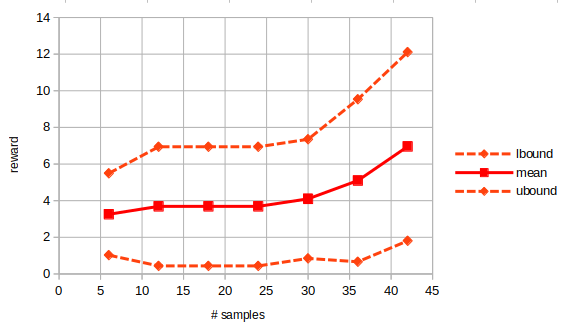
\includegraphics[width=\linewidth]{img/la-mcts.png}
        \caption{LaMCTS with mean and standard deviation}	
    \end{subfigure}
	\hspace{0.02\textwidth}
	\begin{subfigure}[b]{0.3\linewidth}
		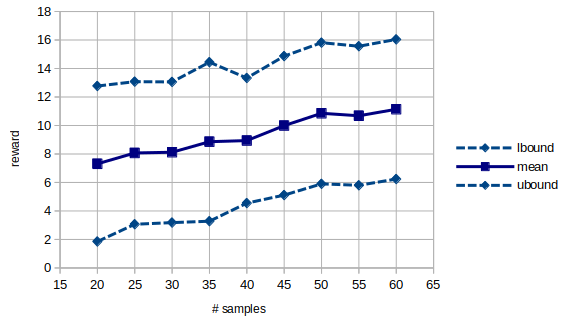
\includegraphics[width=\linewidth]{img/LAP3.png}
		\caption{LAP3 with mean and standard deviation}
	\end{subfigure}
	\hspace{0.02\textwidth}
	\begin{subfigure}[b]{0.3\linewidth}
		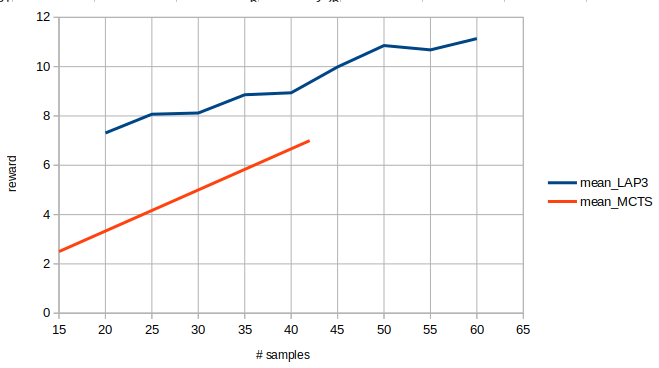
\includegraphics[width=\linewidth]{img/comparison.png}
        \caption{mean of La-MCTS and LAP3}
	\end{subfigure}
	\caption{In maze s3 environment}
	\label{fig:known_problems}
\end{figure}



\begin{figure}[h!]
	\centering
	\begin{subfigure}[b]{0.3\linewidth}
		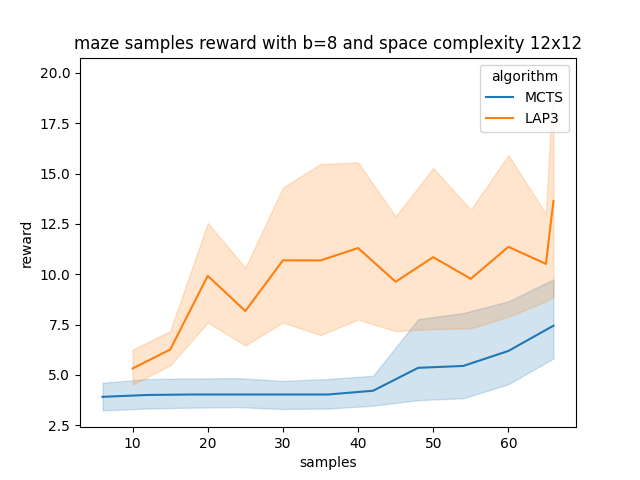
\includegraphics[width=\linewidth]{img/maze_samples__reward_b_8_LAP3_MCTS_12.png}
        \caption{space complexity 12x12}	
    \end{subfigure}
	\hspace{0.02\textwidth}
	\begin{subfigure}[b]{0.3\linewidth}
		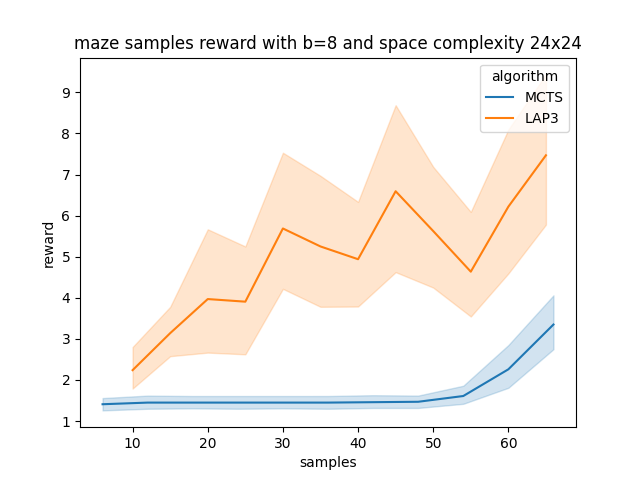
\includegraphics[width=\linewidth]{img/maze_samples__reward_b_8_LAP3_MCTS_24.png}
		\caption{space complexity 24x24}
	\end{subfigure}
	\hspace{0.02\textwidth}
	\begin{subfigure}[b]{0.3\linewidth}
		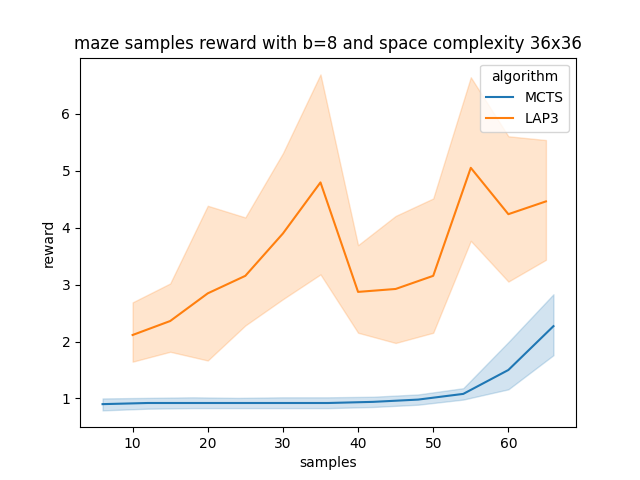
\includegraphics[width=\linewidth]{img/maze_samples__reward_b_8_LAP3_MCTS_36.png}
        \caption{space complexity 36x36}
	\end{subfigure}
	\caption{ratio of samples and reward in Maze s3 environment with different space complexity}
	\label{fig:known_problems}
\end{figure}

\begin{figure}[h!]
	\centering
	\begin{subfigure}[b]{0.3\linewidth}
		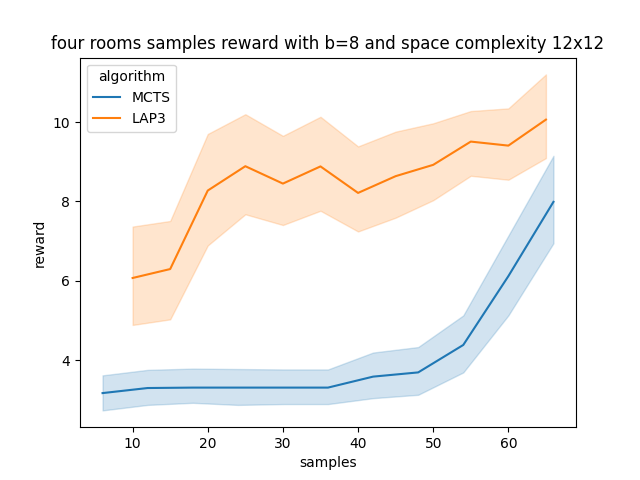
\includegraphics[width=\linewidth]{img/four_rooms_samples__reward_b_8_LAP3_MCTS_12.png}
        \caption{space complexity 12x12}	
    \end{subfigure}
	\hspace{0.02\textwidth}
	\begin{subfigure}[b]{0.3\linewidth}
		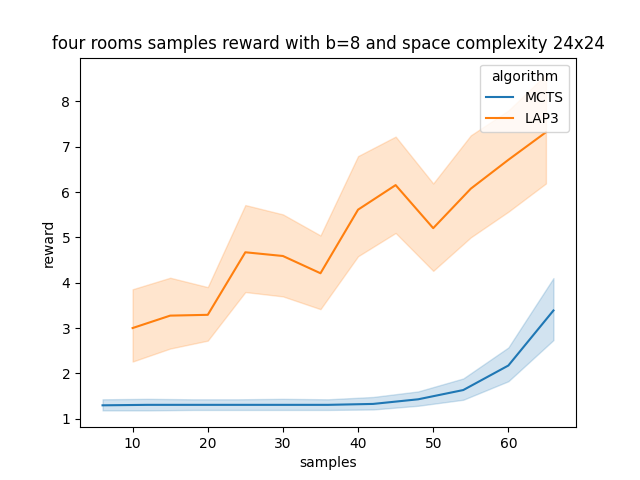
\includegraphics[width=\linewidth]{img/four_rooms_samples__reward_b_8_LAP3_MCTS_24.png}
		\caption{space complexity 24x24}
	\end{subfigure}
	\hspace{0.02\textwidth}
	\begin{subfigure}[b]{0.3\linewidth}
		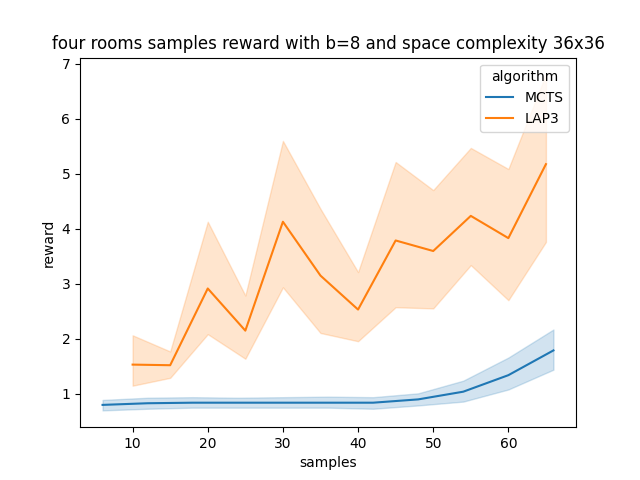
\includegraphics[width=\linewidth]{img/four_rooms_samples__reward_b_8_LAP3_MCTS_36.png}
        \caption{space complexity 36x36}
	\end{subfigure}
	\caption{ratio of samples and reward in four rooms environment with different space complexity}
	\label{fig:known_problems}
\end{figure}


Each algorithm was 

When running each algorithm for 100 times, the 


\section{Conclusions and Further Discussion}

\todo[inline]{What could be explorer in the future}

\clearpage


\section*{Acronyms} 
\addcontentsline{toc}{section}{Acronyms}

\begin{acronym}[....]
    \acro{LaP3}{Latent Space Partitions for Path Planning}
    \acro{MCTS}{Monte Carlo Tree Search}
    \acro{LaMCTS}{Latent Space Monte Carlo Tree Search}
\end{acronym}

\bibliographystyle{alpha}
\bibliography{literature}
\todo[inline]{Alphabetisch sortieren}
\end{document}
